% ------------------------------------------------------------------------------
% Este fichero es parte de la plantilla LaTeX para la realización de Proyectos
% Final de Grado
% ------------------------------------------------------------------------------

Este capítulo trata sobre todos los aspectos relacionados con la implementación en código del sistema \textbf{UniHub}, desglosando la arquitectura técnica de cada una de sus cuatro fases de desarrollo.

\section{Entorno de Construcción}
El marco tecnológico de construcción incluye:
\begin{itemize}
    \item \textbf{Entorno de Desarrollo (IDE):} Visual Studio Code / Antigravity Agent.
    \item \textbf{Lenguajes:} Python 3.12, JavaScript (ES6+ / JSX), SQL (PostgreSQL), HTML5, CSS3.
    \item \textbf{Librerías y Módulos Python:} FastAPI, Uvicorn, SQLAlchemy, Pydantic v2, \texttt{httpx[http2]}, \texttt{h2}, \texttt{requests}, \texttt{psycopg2-binary}, \texttt{xlrd}, \texttt{BeautifulSoup4}, \texttt{pdfplumber}, \texttt{pypdf}, \texttt{psutil}, \texttt{multiprocessing}, \texttt{concurrent.futures}, \texttt{urllib.robotparser}.
    \item \textbf{Librerías y Herramientas JavaScript:} React 19, Vite 8, Oxlint, Lucide React (iconografía UCA), \texttt{usageTracker} analytics, \texttt{perfTracker} performance telemetry.
    \item \textbf{Control de Versiones y Despliegue:} Git, Docker Engine, Docker Compose v2, Nginx 1.25-alpine.
\end{itemize}

\section{Código Fuente y Estructura Modular}
El código fuente del proyecto se organiza de forma modular bajo el directorio \texttt{Codigo/}:

\subsection{Fase 1: Módulo de Ingesta y Crawler (\texttt{Codigo/Crawler/})}
El sistema de ingesta de la Fase 1 se estructura en cuatro partes desacopladas y especializadas:

\subsubsection{Fase 1 - Parte 1: Ingesta del RUCT y Parser PDF del BOE}
\begin{itemize}
    \item \texttt{config.py}: Módulo centralizado de configuración estructurado en 10 secciones temáticas claramente documentadas (Rutas de Archivos, Persistencia Dual, Endpoints Ministeriales del RUCT, Red y Pooling de Conexiones HTTP/2, Circuit Breaker, Paralelismo de Procesos CPU e Hilos I/O, Parámetros de Sitemaps y Robots, Tarifas Públicas SIIU y Privadas, y APIs Externas). Todas las constantes, umbrales, timeouts y retardos admiten sobreescritura dinámica mediante variables de entorno del sistema operativo (\texttt{os.getenv}) con valores de respaldo estandarizados.
    \item \texttt{downloader.py}: Implementa el cliente HTTP resiliente \texttt{RUCTDownloader} con el patrón \emph{Circuit Breaker} y motor dual HTTP/2. Si acumula 10 fallos de red seguidos, se pausa automáticamente durante 5 minutos; si alcanza 3 pausas (15 minutos), lanza \texttt{SkipUniversityException} para omitir la universidad en conflicto sin colapsar el sistema. Incorpora:
    \begin{enumerate}
        \item \textbf{Conexiones Multiplexadas HTTP/2 y Adaptador Transparente (\texttt{HTTP2ResponseWrapper}):} Integración nativa de \texttt{httpx} con soporte HTTP/2 (\texttt{ENABLE\_HTTP2=True}), multiplexación de flujos de datos, compresión binaria de cabeceras HPACK y negociación ALPN automática, con conmutación a HTTP/1.1 cuando el servidor no ofrece HTTP/2. El adaptador expone los métodos de respuesta que emplea el crawler (\texttt{iter\_content}, \texttt{status\_code}, \texttt{headers}, \texttt{raise\_for\_status} y \texttt{close}).
        \item \textbf{Reutilización de Sockets y Keep-Alive Pool:} Pool de conexiones configurado con \texttt{HTTP2\_MAX\_CONNECTIONS=20} y \texttt{HTTP2\_MAX\_KEEPALIVE\_CONNECTIONS=10}, manteniendo canales TLS abiertos hacia los servidores del BOE y ministeriales sin forzar renegociaciones criptográficas continuas.
        \item \textbf{Cerrojo de Concurrencia por Dominio (\texttt{DomainRateLimiter}):} Sincronización mediante cerrojos de hilo por nombre de host (\texttt{\_GLOBAL\_DOMAIN\_LOCKS}) que garantiza que ningún hilo emita peticiones concurrentes contra el mismo dominio universitario a la vez, garantizando un retardo cortés estricto (\texttt{REQUEST\_DELAY = 0.35s} + \emph{Jitter}).
        \item \textbf{Normalización de Enlaces y Verificación de Cabeceras:} Verifica la cabecera mágica \texttt{\%PDF-} en streaming para descartar respuestas HTML erróneas de servidores oficiales, desinfecta esquemas duplicados (\texttt{http://https://}), eleva automáticamente a \texttt{HTTPS} los enlaces de boletines autonómicos (ej. \texttt{dogc.gencat.cat}, \texttt{bocm.madrid.org}, \texttt{doe.juntaex.es}) y corrige de forma canónica erratas tipográficas del ministerio mediante \texttt{DOMAIN\_MAPPINGS} (\texttt{ww.boe.es}, \texttt{vwww.boe.es}, \texttt{wwww.bocm.es}, \texttt{doe.gobex.es}).
    \end{enumerate}
    \item \texttt{parsers.py} y \texttt{boe\_pdf\_parser.py}: Analizan las fichas HTML del RUCT y procesan las resoluciones BOE con un modelo profundo del PDF. El modelo recorre cada página una vez y conserva texto, posiciones de palabras, tablas y delimitadores de titulación. Incorpora:
    \begin{enumerate}
        \item \textbf{Modelo profundo de documento:} Para cada página se reconstruyen líneas a partir de sus coordenadas, se detectan tablas con cabecera curricular y se delimitan secciones cuando una resolución contiene varias titulaciones. Las tablas sin bordes se interpretan desde las líneas posicionadas, sin encadenar estrategias de extracción según el número de filas obtenido.
        \item \textbf{Lectura de documentos escaneados:} Si el PDF carece de capa de texto, el sistema puede aplicar OCR como modalidad de lectura. Si el documento oficial no publica el detalle de asignaturas, el resultado se conserva como incompleto y no se generan filas sintéticas.
        \item \textbf{Priorización contextual de enlaces en RUCT:} Analiza el contexto semántico de cada enlace a BOE en el HTML (leyendas, etiquetas contiguas y texto contenedor) y asigna una prioridad. Las modificaciones de planes y sus publicaciones oficiales prevalecen sobre órdenes generales, acuerdos administrativos, autorizaciones autonómicas o extinciones.
        \item \textbf{Validación de completitud curricular:} Contrasta las filas extraídas con los ECTS declarados y las reglas estructurales aplicables al nivel académico. Esta validación es una señal de calidad; no autoriza a inventar materias que no figuren en una fuente oficial.
        \item \textbf{Fusión Multi-BOE con Cuota por Curso y Parada Temprana:} Algoritmo de integración acumulativa de publicaciones históricas en el BOE que aplica un tope configurable de $60\text{ ECTS}$ por curso académico. La descarga se detiene cuando las comprobaciones de completitud disponibles satisfacen el criterio configurado; la condición se registra como señal de calidad y no sustituye la trazabilidad de las fuentes.
        \item \textbf{Filtro Pre-Bolonia Estricto:} Detección y exclusión automática de resoluciones anteriores a 2009 y planes bajo el Real Decreto derogado 1497/1987.
        \item \textbf{Modelado de Doctorados (RD 99/2011):} Representación específica de programas de doctorado (\texttt{tipo\_estructura: "programa\_doctorado\_investigacion"}) registrando líneas de investigación, tutela académica anual y descartando asignaturas lectivas ficticias.
        \item \textbf{Normalización de curso y cuatrimestre:} Algoritmos deterministas acotan los cursos a los valores admisibles y normalizan los periodos a primer cuatrimestre, segundo cuatrimestre o anualidad. También corrigen desplazamientos producidos por la maquetación tabular.
        \item \textbf{Saneamiento Transversal Universal (\texttt{sanitize\_string\_value}):} Limpieza sistemática aplicada en todos los niveles (universidades, titulaciones, módulos, materias y nombres de asignaturas), corrigiendo textos invertidos de tipografías históricas (\texttt{unreverse\_text}), colapsando espacios múltiples, eliminando caracteres de control invisibles y suprimiendo puntuación residual huérfana al final de cadena (\texttt{.rstrip(".:;,")}).
    \end{enumerate}
    \item \texttt{fase1\_parte1\_ruct\_boe.py}: Orquesta la ejecución mediante una arquitectura paralela Productor-Consumidor con buffer híbrido en memoria:
    \begin{enumerate}
        \item \textbf{Buffer Híbrido en Memoria y Spill-to-Disk (\texttt{MAX\_IN\_MEMORY\_PDF\_BYTES = 5 MB}):} Los PDFs con tamaño $\le 5\text{ MB}$ se transmiten directamente en la cola de tareas multiproceso en memoria RAM como secuencias de bytes (\texttt{pdf\_bytes}), eliminando por completo el I/O en disco. Los PDFs excepcionales $> 5\text{ MB}$ aplican volcado temporal a disco con garantía estricta de borrado en bloques \texttt{finally}.
        \item \textbf{Precargador asíncrono acotado:} Un ejecutor de hilos, limitado por la configuración, adelanta los metadatos de un máximo de tres titulaciones. De este modo se solapan las esperas de red con el análisis de PDF, manteniendo el cerrojo de cortesía por dominio.
    \end{enumerate}
\end{itemize}

\begin{figure}[htbp]
    \centering
    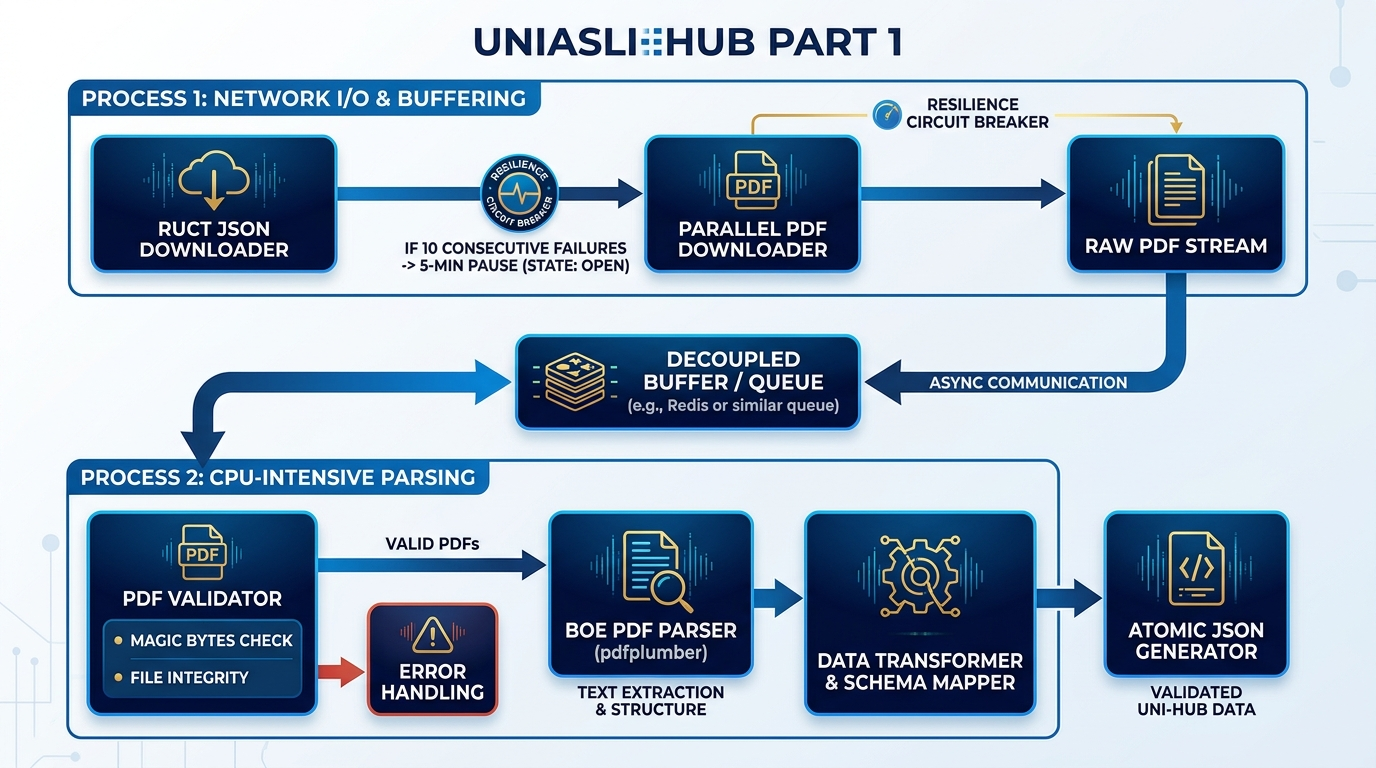
\includegraphics[width=0.92\textwidth]{figures/fase1_parte1_diagram.jpg}
    \caption{Diagrama de arquitectura paralela Productor-Consumidor y resiliencia Circuit Breaker de la Fase 1 Parte 1}
    \label{fig:fase1_parte1_diagram}
\end{figure}

\subsubsection{Fase 1 - Parte 2: Recuperación desde Webs Oficiales}
\begin{itemize}
    \item \texttt{fase1\_parte2\_web\_crawler.py}: Rastreado de portales oficiales para titulaciones sin plan BOE o con información incompleta. Normaliza protocolos HTTPS, comprueba \texttt{robots.txt}, aplica \texttt{Crawl-delay} cuando se publica y consulta mapas de sitio \texttt{sitemap.xml}.
    \item \textbf{Índice Hub-and-Spoke con BFS multinivel:} Sistema de preindexación en cascada mediante recorrido en anchura (\emph{Breadth-First Search}, BFS) sobre catálogos maestros, facultades y portales de calidad. El número de nodos y saltos se limita mediante parámetros configurables, al igual que la profundidad de las URL. Los enlaces a titulaciones se normalizan con Unicode NFKD y formas en singular y plural para priorizar la ficha docente más pertinente.
        \item \textbf{Priorización de memorias verificadas:} Los documentos institucionales de acreditación reciben prioridad semántica. Su contenido se somete a los mismos filtros de identidad, estructura curricular y calidad; la prioridad no supone una garantía automática de cobertura total.
    \item \textbf{Garantía de Rastreo Secuencial y Cortesía Monodominio:} La exploración de los catálogos y de las subpáginas docentes se realiza de forma estrictamente secuencial sobre cada universidad, respetando el retardo cortés oficial (\texttt{REQUEST\_DELAY = 0.35s} y dispersión aleatoria \emph{Jitter}), garantizando que ningún servidor institucional reciba peticiones simultáneas desde el mismo cliente.
    \item \textbf{Disparo de Descarga Automática en Navegador (\emph{Playwright Download Trigger}):} Manejo especializado de enlaces de facultades que disparan descargas binarias automáticas (\texttt{Download is starting} / \texttt{net::ERR\_ABORTED}) mediante la subclase \texttt{RenderResult} en \texttt{spa\_crawler.py}, interceptando los flujos de bytes del PDF en memoria y procesándolos con \texttt{parse\_boe\_pdf()}.
    \item \textbf{Disparo Condicional Inteligente de Renderizado SPA (Playwright):} El motor de navegador sin cabeza (\emph{headless} Chromium) solo se instancia cuando el HTML estático carece de materias curriculares ($< 3\text{ asignaturas}$), evitando cargar un navegador en páginas institucionales convencionales basadas en HTML estático.
    \item \textbf{Ruta Rápida de Resolución HTML:} Reutiliza las URLs identificadas en ejecuciones anteriores para evitar redescubrimientos innecesarios, siempre que la respuesta y su fuente superen las validaciones establecidas.
    \item \textbf{Filtros Defensivos Anti-Tablas Administrativas y Soporte Multilingüe:} Implementa cuatro barreras matemáticas en \texttt{extract\_html\_subjects} para descartar tablas no curriculares (horarios, comisiones, baremos de ponderación, calendarios de exámenes) mediante la expresión regular \texttt{RE\_SUMMARY\_LABEL} y acotando los créditos por asignatura a $\le 30\text{ ECTS}$. Cuenta con soporte semántico para lenguas cooficiales (catalán, valenciano, gallego, euskera e inglés).
    \item \textbf{Descubrimiento Orgánico de Centros Adscritos y Alianzas Europeas:} Sistema de detección autónoma de hiperenlaces salientes a centros concertados (\texttt{centres adscrits}, escuelas de negocios, diseño y hostelería como CETT o ESCAC) y consorcios internacionales (\emph{SEA-EU, EUNICE, CHARM-EU, Arqus, Erasmus Mundus}) presentes de forma natural en las páginas de oferta formativa de la universidad matriz, indexando dichos sub-hubs al vuelo con \texttt{DomainRateLimiter} independiente y sin requerir listas estáticas de URLs en archivos de configuración.
    \item \textbf{Ficha de Consorcio Internacional Erasmus Mundus / Alianzas Europeas:} Estructura automáticamente la acreditación oficial de másteres conjuntos internacionales cuya docencia se gestiona en portales europeos multilingües, asignando la carga oficial de créditos ECTS verificada por ANECA y enlazando al portal del consorcio europeo.
    \item \textbf{Extracción Tarifaria Privada:} Captura precios oficiales por crédito ECTS e importes anuales mediante expresiones regulares en universidades privadas (\texttt{extract\_private\_university\_pricing()}), respetando la política estricta de no inyectar valores ficticios.
\end{itemize}

\begin{figure}[htbp]
    \centering
    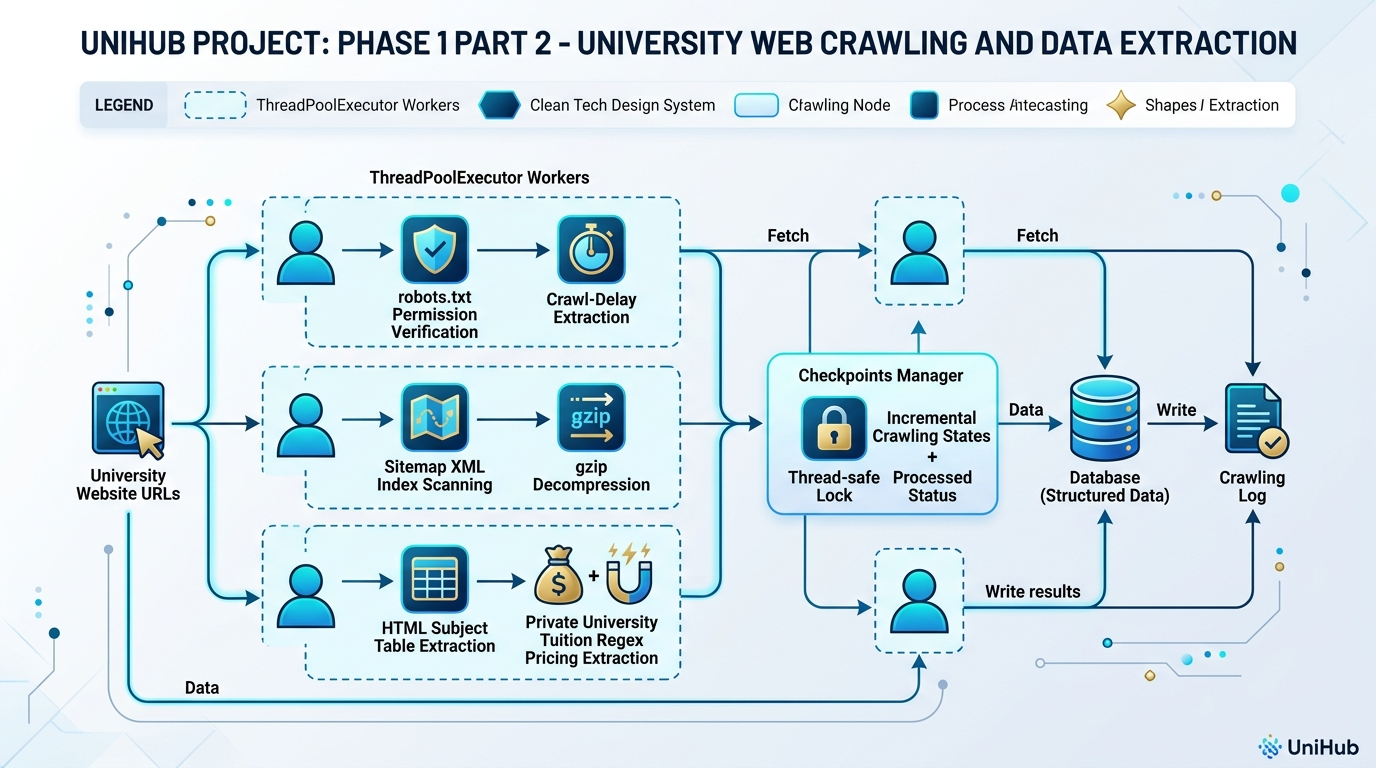
\includegraphics[width=0.92\textwidth]{figures/fase1_parte2_diagram.jpg}
    \caption{Flujo de rastreo web oficial con arquitectura Hub-and-Spoke, verificación robots.txt, sitemaps XML y extracción tarifaria privada de la Fase 1 Parte 2}
    \label{fig:fase1_parte2_diagram}
\end{figure}

\subsubsection{Fase 1 - Parte 3: Consolidación de Precios Públicos ECTS (SIIU)}
\begin{itemize}
    \item \texttt{fase1\_parte3\_precios.py}: Asigna precios públicos por crédito ECTS e importes anuales estimados a partir del catálogo local de referencias SIIU y normativa autonómica disponible.
    \item Dispone de un catálogo local pre-cargado \texttt{OFFICIAL\_SIIU\_PRICES\_CATALOG} para las 17 Comunidades Autónomas más la UNED. Sus importes deben verificarse contra la normativa vigente antes de una liquidación real.
    \item Implementa discriminación por categoría (\emph{Grado, Máster Habilitante, Máster No Habilitante y Doctorado}) con la fórmula anual base $\text{Coste} = (60 \text{ ECTS} \times \text{Precio ECTS}) + \text{Tasas Admin}$.
    \item Incorpora \textbf{caché en memoria} del catálogo \texttt{precios\_ccaa.json} y volcado atómico mediante \texttt{atomic\_json\_dump} sobre los planes de estudio y el índice de titulaciones.
\end{itemize}

\begin{figure}[htbp]
    \centering
    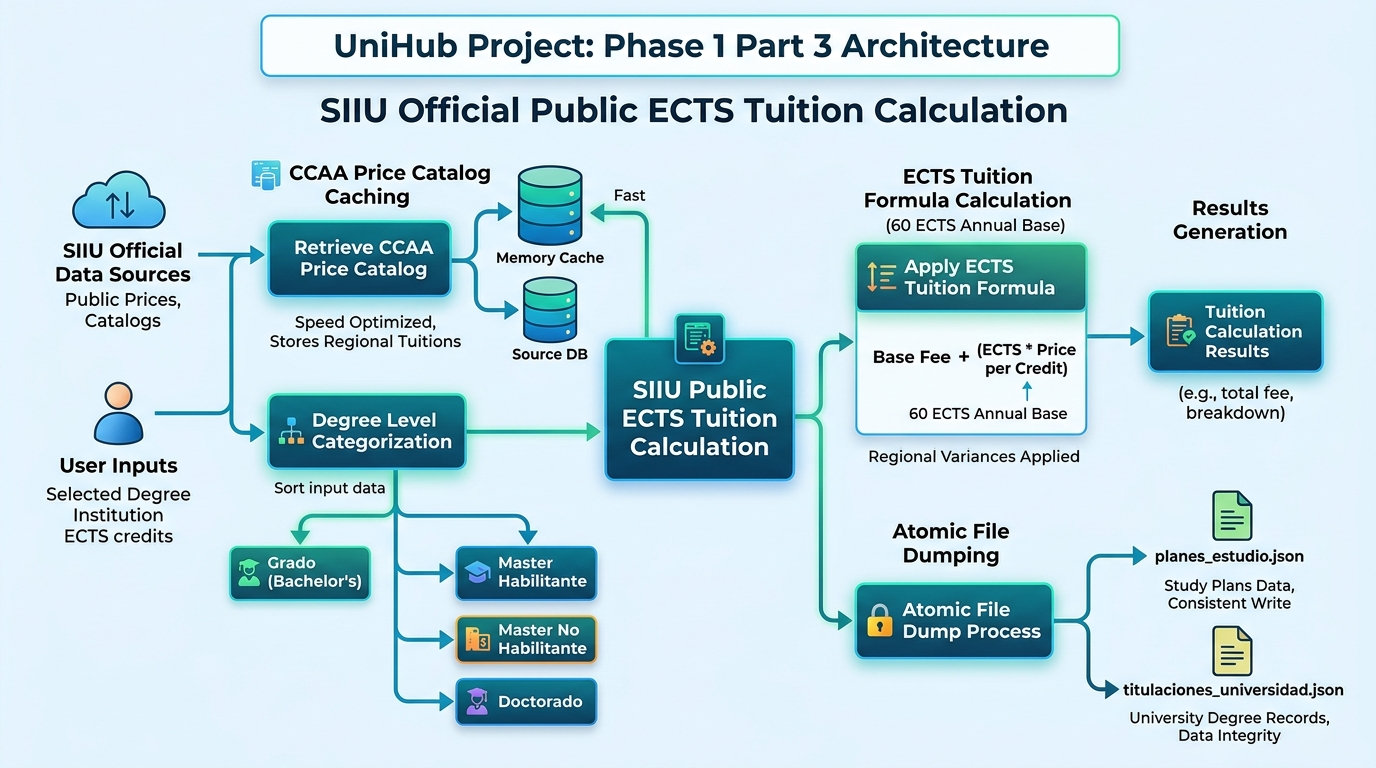
\includegraphics[width=0.92\textwidth]{figures/fase1_parte3_diagram.jpg}
    \caption{Algoritmo de cómputo tarifario a partir del catálogo local, cacheo en memoria RAM y sincronización de la Fase 1 Parte 3}
    \label{fig:fase1_parte3_diagram}
\end{figure}

\subsubsection{Fase 1 - Parte 4: Guías Docentes y Temarios EEES (\texttt{fase1\_parte4\_asignaturas.py})}
\begin{itemize}
    \item \texttt{fase1\_parte4\_asignaturas.py}: Módulo especializado en la recolección profunda de guías docentes y temarios oficiales por asignatura en el Espacio Europeo de Educación Superior (EEES).
    \item Extrae descriptores de competencias, resultados de aprendizaje, criterios de evaluación y bloques temáticos por asignatura, enlazando la guía docente digitalizada al plan de estudios correspondiente.
    \item Utiliza el motor de saneamiento \texttt{is\_spurious\_or\_administrative\_subject} para filtrar materias administrativas o residuales, garantizando un enriquecimiento limpio y coherente.
\end{itemize}

\subsubsection{Gestor de Estado Incremental (\texttt{CheckpointManager})}
\begin{itemize}
    \item \texttt{checkpoint.py}: Gestor atómico del estado del rastreo. Mantiene el estado de reanudación en \texttt{checkpoint.json} y utiliza SQLite WAL para el ledger de peticiones y la caché. La escritura se agrupa en puntos de control para evitar operaciones de disco innecesarias.
\end{itemize}

\subsubsection{Mecanismos de Rendimiento, Reanudación y Cortesía}
La Fase 1 incorpora mecanismos orientados a reducir trabajo repetido sin alterar la semántica de los datos ni el comportamiento respetuoso frente a los servidores externos:
\begin{itemize}
    \item \textbf{Paralelismo acotado:} La Parte 1 desacopla descargas y análisis de PDF mediante trabajadores configurables. La precarga RUCT se limita por \texttt{ASYNC\_PREFETCH\_WORKERS} y \texttt{RUCT\_PREFETCH\_LOOKAHEAD}.
    \item \textbf{Transferencia híbrida de PDF:} Los documentos pequeños se procesan en memoria y los que superan el umbral \texttt{MAX\_IN\_MEMORY\_PDF\_BYTES} se gestionan temporalmente en disco con limpieza garantizada.
    \item \textbf{Modelo profundo de PDF:} El parser abre el documento una vez para reunir geometría, tablas y texto. La selección de filas se basa en cabeceras curriculares y en la sección de la titulación, reduciendo tanto duplicados como falsos positivos administrativos.
    \item \textbf{Caché y ledger:} Las respuestas HTTP, sus validadores y huellas SHA-256 se registran en SQLite WAL. Esto permite reanudar y revalidar fuentes sin repetir solicitudes cuando la caché es válida.
    \item \textbf{Rastreo web responsable:} Las Partes 2 y 4 agrupan el trabajo por universidad, consultan \texttt{robots.txt}, respetan retardos por dominio y aplican límites de profundidad y de tamaño de respuesta.
    \item \textbf{Renderizado condicional:} Playwright se reserva para portales cuyo HTML estático no aporta información curricular suficiente, con el objetivo de no cargar un navegador para páginas convencionales.
\end{itemize}

\subsection{Fase 2: Módulo de API REST y Persistencia (\texttt{Codigo/API/})}
\begin{itemize}
    \item \texttt{database/schema.sql}: Define el esquema relacional en PostgreSQL. Activa la extensión de trigramas \texttt{pg\_trgm} con índices GIN en columnas de búsqueda (\texttt{nombre}, \texttt{titulo}) y crea el rol restringido \texttt{unihub\_api\_user}. Incorpora las columnas de trazabilidad y desduplicación \texttt{origen\_fuente} y \texttt{pdf\_sha256} en la tabla \texttt{planes\_estudio}.
    \item \texttt{connection.py}: Gestiona el conjunto de conexiones SQLAlchemy (\texttt{pool\_size=15}, \texttt{max\_overflow=25}, \texttt{pool\_pre\_ping=True}).
    \item \texttt{security.py}: Control de acceso administrativo para la cabecera HTTP \texttt{X-API-Key}. Valida la clave mediante \texttt{secrets.compare\_digest(api\_key, settings.ADMIN\_API\_KEY)}, inmune a ataques de tiempo (timing attacks) por canal lateral.
    \item \texttt{etl\_loader.py}: Proceso de ingesta de datos JSON hacia la base de datos utilizando \texttt{bulk\_save\_objects} para acelerar las inserciones masivas de asignaturas (reduciendo el tiempo de 15s a menos de 1.5s). Soporta rutas adaptativas tanto en entorno nativo como contenerizado (\texttt{/app/Datos}). Incorpora un mecanismo de sincronización reactiva en segundo plano con control de concurrencia mediante archivo de cerrojo de proceso PID (\texttt{etl\_running.lock} en \texttt{tempfile.gettempdir()}) y comprobación de PID activo con \texttt{os.kill(pid, 0)}. Incluye un umbral de seguridad de representatividad ($\ge 100$ titulaciones) para prevenir borrados en cascada accidentales ante volcados parciales del crawler.
    \item \texttt{routes/}: Define los controladores REST para universidades (\texttt{universidades.py}), titulaciones y planes (\texttt{titulaciones.py}) y telemetría (\texttt{estadisticas.py}). Destaca el soporte para filtrado vocacional por Rama de Conocimiento (\texttt{rama}: \emph{sociales, ingenieria, salud, humanidades, ciencias}), el endpoint \texttt{GET /api/v1/estadisticas/cobertura} que expone la cobertura global y el validador \texttt{GET /api/v1/auth/verify}.
\end{itemize}

\subsection{Fase 3: Módulo de Interfaz Web y Calculadora (\texttt{Codigo/WWW/})}
\begin{itemize}
    \item \texttt{src/components/ErrorBoundary.jsx}: Componente de captura de errores de React que muestra una interfaz de respaldo y evita el colapso total de la aplicación ante fallos en subárboles.
    \item \texttt{src/components/AdminLogin.jsx}: Acceso asegurado con validación asíncrona en tiempo real contra el endpoint \texttt{/auth/verify} del backend antes de transicionar al panel de control, con indicador de carga animado.
    \item Carga diferida de rutas pesadas con \texttt{React.lazy} y \texttt{Suspense}: \texttt{AdminDashboard}, \texttt{AdminLogin}, \texttt{Geolocation}, \texttt{TuitionCalculator}, \texttt{AboutUs}, \texttt{Pagination} y \texttt{Footer} se cargan bajo demanda para reducir el bundle inicial.
    \item \texttt{src/services/api.js}: Cliente de comunicación HTTP con la API REST con interceptor de latencias \texttt{perfTracker}, propagación del filtro \texttt{rama}, filtrado de excepciones \texttt{AbortError} (para no distorsionar métricas en búsquedas con *debounce*) y formateo corregido de CCAA.
    \item \texttt{src/App.jsx}: Enrutamiento SPA sincronizado con la \textbf{History API} del navegador (\texttt{pushState} y escucha de eventos \texttt{popstate}), permitiendo la navegación fluida y el soporte nativo del botón atrás/adelante. Incorpora el banner interactivo de desconexión (\emph{Offline Alert Banner}) con detección en tiempo real de fallos de red hacia el backend y botón de reintento de conexión inmediato.
    \item \texttt{src/components/PlanModal.jsx}: Modal curricular con tarjeta específica para Doctorados bajo RD 99/2011, bloqueo de scroll en el body (\texttt{overflow: hidden}) y resaltado visual de \textbf{Menciones Curriculares e Itinerarios Oficiales} (\texttt{[Menci\'on...]}) para más de 420 grados.
    \item \texttt{src/components/Navbar.jsx}: Barra de navegación accesible con soporte para menú hamburguesa táctil colapsable en dispositivos móviles y conmutador de modo claro/oscuro.
    \item \texttt{src/components/TuitionCalculator.jsx}: Motor de simulación financiera de matrícula universitaria. Implementa multiplicadores por repetición de asignatura ($1.0\times, 1.5\times, 3.0\times, 4.5\times$), selección rápida por curso, preselección segura hasta 60 ECTS para planes planos, soporte para universidades públicas y privadas, y el sistema completo de exenciones sociales (Beca MEC, Familia Numerosa, Discapacidad $\ge 33\%$, Bonificación 99\% CCAA y Matrícula de Honor).
    \item \texttt{src/components/Geolocation.jsx}: Búsqueda de universidades por distancia Haversine a más de 50 ciudades y capitales de provincia de España o ubicación GPS con reinicio automático de paginación.
    \item \texttt{src/components/AboutUs.jsx}: Sección informativa ampliada con el desglose técnico de las 4 Fases, datos institucionales del TFG de la UCA y enlaces interactivos a fuentes oficiales.
    \item \texttt{src/components/AdminDashboard.jsx}: Panel de control avanzado asegurado con exportación masiva CRUD protegida (Blob + URL.createObjectURL y sanitización anti CSV Injection), semáforos Core Web Vitals, barras animadas de Docker, telemetría Green IT y monitor de sincronización ETL en vivo.
    \item \texttt{src/components/DegreeCard.jsx} y \texttt{UnivCard.jsx}: Componentes visuales memoizados con soporte de accesibilidad por teclado (\texttt{tabIndex=\{0\}}, eventos de tecla \texttt{Enter}/\texttt{Espacio}), parseo numérico protegido y cálculo instantáneo de costes de 1ª a 4ª matrícula.
    \item \texttt{src/index.css}: Sistema de diseño basado en la identidad corporativa de la Universidad de Cádiz (UCA) con variables CSS, efectos \emph{glassmorphism}, scrollbar estándar multiplataforma (\texttt{scrollbar-width: thin}) y adaptabilidad responsive integral.
\end{itemize}

\subsection{Fase 4: Despliegue Contenerizado y Orquestación (\texttt{Codigo/Docker/})}
\begin{itemize}
    \item \texttt{docker-compose.yml}: Define la red interna \texttt{unihub\_network}, el volumen persistente \texttt{unihub\_postgres\_data} y los 4 servicios (\texttt{db}, \texttt{crawler}, \texttt{api}, \texttt{www}). Incluye \texttt{healthcheck} con \texttt{pg\_isready} para la base de datos y verificación de estado en la API (\texttt{/api/v1/salud}); el servicio web depende del estado saludable declarado por la API (\texttt{condition: service\_healthy}).
    \item \texttt{api/Dockerfile}: Imagen base \texttt{python:3.12-slim}. Instala dependencias de sistema \texttt{postgresql-client}, \texttt{libpq-dev}, \texttt{gcc}, \texttt{g++} y copia \texttt{Codigo/API} y \texttt{Codigo/Crawler/Datos} al contenedor.
    \item \texttt{crawler/Dockerfile}: Imagen base Python con volumen montado \texttt{/app/Datos}. Copia todo el crawler para ejecutar \texttt{main.py} de forma programada o manual.
    \item \texttt{www/Dockerfile}: Construcción multi-etapa Node 20-alpine para el build Vite y Nginx 1.25-alpine para servir los artefactos estáticos. Variables \texttt{VITE\_API\_URL}, \texttt{VITE\_ADMIN\_USER}, \texttt{VITE\_ADMIN\_FEES} inyectadas en compilación.
    \item \texttt{entrypoint.sh}: Script de arranque que comprueba la disponibilidad de PostgreSQL mediante \texttt{nc} y lanza el servidor FastAPI con \texttt{uvicorn main:app --host 0.0.0.0 --port 8000}.
\end{itemize}

\subsection{Pruebas y Auditoría de Rendimiento (\texttt{Codigo/Pruebas/})}
\begin{itemize}
    \item \texttt{run\_phase1\_detailed\_test.py}: Prueba de trazabilidad y auditoría sobre 5 universidades de referencia (3 públicas y 2 privadas). Ejecuta Parte 1 RUCT+BOE PDF, Parte 2 rescate web oficial y Wikidata, Parte 3 cálculo de precios ECTS. Genera informe Markdown y JSON con métricas de cobertura, asignaturas extraídas y auditoría de redundancias.
    \item Detección de redundancias: RED-01 normalización duplicada de URLs en \texttt{downloader.py} y \texttt{parsers.py}; RED-02 lecturas repetidas de \texttt{plan\_file} en \texttt{univ\_web\_crawler.py}, \texttt{main.py} y \texttt{precios\_crawler.py}; RED-03 recálculo de precios en múltiples pasos.
    \item Documentación de pruebas: \texttt{EstudioRendimientoFase1.md}, \texttt{EstudioTasaAciertoReal.md}, \texttt{ResultadosPruebaFase1.md/json}.
\end{itemize}

\begin{figure}[htbp]
    \centering
    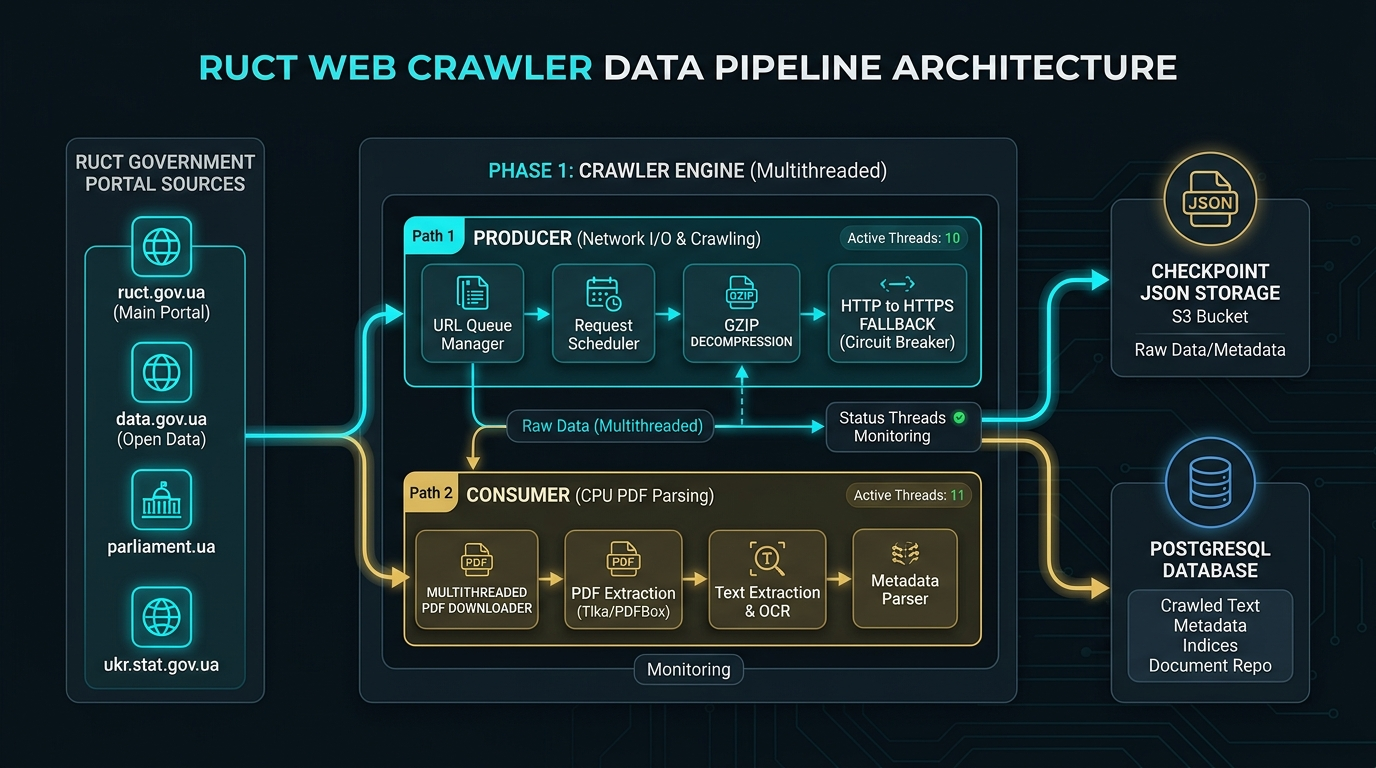
\includegraphics[width=0.95\textwidth]{figures/unihub_crawler_architecture.jpg}
    \caption{Diagrama de arquitectura paralela Productor-Consumidor y resiliencia de red de la Fase 1}
    \label{fig:crawler_architecture}
\end{figure}

\section{Código DDL de Base de datos}
El esquema físico en PostgreSQL se construye mediante el archivo DDL \texttt{schema.sql}:
\begin{lstlisting}[language=SQL, caption={Esquema DDL relacional, tabla planes\_estudio y rol de solo lectura de la API}]
CREATE TABLE IF NOT EXISTS universidades (
    id SERIAL PRIMARY KEY,
    codigo VARCHAR(10) UNIQUE NOT NULL,
    nombre VARCHAR(500) NOT NULL,
    tipo VARCHAR(50),
    comunidad_autonoma VARCHAR(100),
    municipio VARCHAR(100),
    provincia VARCHAR(100),
    web VARCHAR(500),
    email VARCHAR(255),
    telefono VARCHAR(50),
    creado_en TIMESTAMP DEFAULT CURRENT_TIMESTAMP
);

CREATE TABLE IF NOT EXISTS titulaciones (
    id SERIAL PRIMARY KEY,
    codigo_estudio VARCHAR(20) UNIQUE NOT NULL,
    universidad_codigo VARCHAR(10) REFERENCES universidades(codigo),
    titulo VARCHAR(255) NOT NULL,
    nivel_academico VARCHAR(50),
    estado VARCHAR(200),
    precio_credito_ects NUMERIC(10,2),
    precio_estimado_anual NUMERIC(10,2),
    fuente_precio VARCHAR(100),
    creado_en TIMESTAMP DEFAULT CURRENT_TIMESTAMP
);

CREATE TABLE IF NOT EXISTS planes_estudio (
    id SERIAL PRIMARY KEY,
    codigo_estudio VARCHAR(20) UNIQUE REFERENCES titulaciones(codigo_estudio) ON DELETE CASCADE,
    boe_url TEXT,
    boe_fecha DATE,
    origen_fuente VARCHAR(100),
    pdf_sha256 VARCHAR(64),
    fecha_procesado TIMESTAMP,
    creado_en TIMESTAMP DEFAULT CURRENT_TIMESTAMP
);

-- Rol de solo lectura para la API REST (Soporte dinamico en inicializacion Docker)
DO
$do$
BEGIN
   IF NOT EXISTS (
      SELECT FROM pg_catalog.pg_roles
      WHERE  rolname = 'unihub_api_user') THEN
      CREATE ROLE unihub_api_user WITH LOGIN PASSWORD '${POSTGRES_API_PASSWORD}';
   END IF;
END
$do$;

EXECUTE format('GRANT CONNECT ON DATABASE %I TO unihub_api_user', current_database());
GRANT USAGE ON SCHEMA public TO unihub_api_user;
GRANT SELECT ON ALL TABLES IN SCHEMA public TO unihub_api_user;
ALTER DEFAULT PRIVILEGES IN SCHEMA public GRANT SELECT ON TABLES TO unihub_api_user;
\end{lstlisting}
